% Options for packages loaded elsewhere
\PassOptionsToPackage{unicode}{hyperref}
\PassOptionsToPackage{hyphens}{url}
\PassOptionsToPackage{dvipsnames,svgnames*,x11names*}{xcolor}
%
\documentclass[
]{book}
\usepackage{lmodern}
\usepackage{amsmath}
\usepackage{ifxetex,ifluatex}
\ifnum 0\ifxetex 1\fi\ifluatex 1\fi=0 % if pdftex
  \usepackage[T1]{fontenc}
  \usepackage[utf8]{inputenc}
  \usepackage{textcomp} % provide euro and other symbols
  \usepackage{amssymb}
\else % if luatex or xetex
  \usepackage{unicode-math}
  \defaultfontfeatures{Scale=MatchLowercase}
  \defaultfontfeatures[\rmfamily]{Ligatures=TeX,Scale=1}
\fi
% Use upquote if available, for straight quotes in verbatim environments
\IfFileExists{upquote.sty}{\usepackage{upquote}}{}
\IfFileExists{microtype.sty}{% use microtype if available
  \usepackage[]{microtype}
  \UseMicrotypeSet[protrusion]{basicmath} % disable protrusion for tt fonts
}{}
\makeatletter
\@ifundefined{KOMAClassName}{% if non-KOMA class
  \IfFileExists{parskip.sty}{%
    \usepackage{parskip}
  }{% else
    \setlength{\parindent}{0pt}
    \setlength{\parskip}{6pt plus 2pt minus 1pt}}
}{% if KOMA class
  \KOMAoptions{parskip=half}}
\makeatother
\usepackage{xcolor}
\IfFileExists{xurl.sty}{\usepackage{xurl}}{} % add URL line breaks if available
\IfFileExists{bookmark.sty}{\usepackage{bookmark}}{\usepackage{hyperref}}
\hypersetup{
  pdftitle={Estatística \& Probabilidade aplicado às Engenharias e Ciências},
  pdfauthor={Ben Dêivide de Oliveira Batista},
  colorlinks=true,
  linkcolor=Maroon,
  filecolor=Maroon,
  citecolor=Blue,
  urlcolor=Blue,
  pdfcreator={LaTeX via pandoc}}
\urlstyle{same} % disable monospaced font for URLs
\usepackage{color}
\usepackage{fancyvrb}
\newcommand{\VerbBar}{|}
\newcommand{\VERB}{\Verb[commandchars=\\\{\}]}
\DefineVerbatimEnvironment{Highlighting}{Verbatim}{commandchars=\\\{\}}
% Add ',fontsize=\small' for more characters per line
\usepackage{framed}
\definecolor{shadecolor}{RGB}{248,248,248}
\newenvironment{Shaded}{\begin{snugshade}}{\end{snugshade}}
\newcommand{\AlertTok}[1]{\textcolor[rgb]{0.33,0.33,0.33}{#1}}
\newcommand{\AnnotationTok}[1]{\textcolor[rgb]{0.37,0.37,0.37}{\textbf{\textit{#1}}}}
\newcommand{\AttributeTok}[1]{\textcolor[rgb]{0.61,0.61,0.61}{#1}}
\newcommand{\BaseNTok}[1]{\textcolor[rgb]{0.06,0.06,0.06}{#1}}
\newcommand{\BuiltInTok}[1]{#1}
\newcommand{\CharTok}[1]{\textcolor[rgb]{0.5,0.5,0.5}{#1}}
\newcommand{\CommentTok}[1]{\textcolor[rgb]{0.37,0.37,0.37}{\textit{#1}}}
\newcommand{\CommentVarTok}[1]{\textcolor[rgb]{0.37,0.37,0.37}{\textbf{\textit{#1}}}}
\newcommand{\ConstantTok}[1]{\textcolor[rgb]{0,0,0}{#1}}
\newcommand{\ControlFlowTok}[1]{\textcolor[rgb]{0.27,0.27,0.27}{\textbf{#1}}}
\newcommand{\DataTypeTok}[1]{\textcolor[rgb]{0.27,0.27,0.27}{#1}}
\newcommand{\DecValTok}[1]{\textcolor[rgb]{0.06,0.06,0.06}{#1}}
\newcommand{\DocumentationTok}[1]{\textcolor[rgb]{0.37,0.37,0.37}{\textbf{\textit{#1}}}}
\newcommand{\ErrorTok}[1]{\textcolor[rgb]{0.14,0.14,0.14}{\textbf{#1}}}
\newcommand{\ExtensionTok}[1]{#1}
\newcommand{\FloatTok}[1]{\textcolor[rgb]{0.06,0.06,0.06}{#1}}
\newcommand{\FunctionTok}[1]{\textcolor[rgb]{0,0,0}{#1}}
\newcommand{\ImportTok}[1]{#1}
\newcommand{\InformationTok}[1]{\textcolor[rgb]{0.37,0.37,0.37}{\textbf{\textit{#1}}}}
\newcommand{\KeywordTok}[1]{\textcolor[rgb]{0.27,0.27,0.27}{\textbf{#1}}}
\newcommand{\NormalTok}[1]{#1}
\newcommand{\OperatorTok}[1]{\textcolor[rgb]{0.43,0.43,0.43}{\textbf{#1}}}
\newcommand{\OtherTok}[1]{\textcolor[rgb]{0.37,0.37,0.37}{#1}}
\newcommand{\PreprocessorTok}[1]{\textcolor[rgb]{0.37,0.37,0.37}{\textit{#1}}}
\newcommand{\RegionMarkerTok}[1]{#1}
\newcommand{\SpecialCharTok}[1]{\textcolor[rgb]{0,0,0}{#1}}
\newcommand{\SpecialStringTok}[1]{\textcolor[rgb]{0.5,0.5,0.5}{#1}}
\newcommand{\StringTok}[1]{\textcolor[rgb]{0.5,0.5,0.5}{#1}}
\newcommand{\VariableTok}[1]{\textcolor[rgb]{0,0,0}{#1}}
\newcommand{\VerbatimStringTok}[1]{\textcolor[rgb]{0.5,0.5,0.5}{#1}}
\newcommand{\WarningTok}[1]{\textcolor[rgb]{0.37,0.37,0.37}{\textbf{\textit{#1}}}}
\usepackage{longtable,booktabs}
\usepackage{calc} % for calculating minipage widths
% Correct order of tables after \paragraph or \subparagraph
\usepackage{etoolbox}
\makeatletter
\patchcmd\longtable{\par}{\if@noskipsec\mbox{}\fi\par}{}{}
\makeatother
% Allow footnotes in longtable head/foot
\IfFileExists{footnotehyper.sty}{\usepackage{footnotehyper}}{\usepackage{footnote}}
\makesavenoteenv{longtable}
\usepackage{graphicx}
\makeatletter
\def\maxwidth{\ifdim\Gin@nat@width>\linewidth\linewidth\else\Gin@nat@width\fi}
\def\maxheight{\ifdim\Gin@nat@height>\textheight\textheight\else\Gin@nat@height\fi}
\makeatother
% Scale images if necessary, so that they will not overflow the page
% margins by default, and it is still possible to overwrite the defaults
% using explicit options in \includegraphics[width, height, ...]{}
\setkeys{Gin}{width=\maxwidth,height=\maxheight,keepaspectratio}
% Set default figure placement to htbp
\makeatletter
\def\fps@figure{htbp}
\makeatother
\setlength{\emergencystretch}{3em} % prevent overfull lines
\providecommand{\tightlist}{%
  \setlength{\itemsep}{0pt}\setlength{\parskip}{0pt}}
\setcounter{secnumdepth}{5}
\ifluatex
  \usepackage{selnolig}  % disable illegal ligatures
\fi
\usepackage[]{natbib}
\bibliographystyle{apalike}

\title{Estatística \& Probabilidade aplicado às Engenharias e Ciências}
\author{Ben Dêivide de Oliveira Batista}
\date{2021-05-07}

\begin{document}
\maketitle

{
\hypersetup{linkcolor=}
\setcounter{tocdepth}{2}
\tableofcontents
}
\listoftables
\listoffigures
\textless! -

\hypertarget{bem-vindo}{%
\chapter*{Bem-vindo}\label{bem-vindo}}


Esse é um \emph{livro digital} da 1ª edição do \textbf{``\href{}{Estatística \& Probabilidade aplicado às Engenharias e Ciências}''}, um livro com o selo \textbf{Democratizando Conhecimento} (\textbf{DC}). O Livro é voltado para quem deseja iniciar no estudo sobre a estatística. Daremos as bases e fundamentos, de modo aplicado a problemas na área das Engenharias e Ciências, de assuntos desde o que é uma população, amostra, até estudos sobre a teoria de decisão, estudo de regressão, dentre outros assuntos básicos, para que assim, a partir desse material, o leitor tenha base para ler, assuntos mais aprofundados na área da estatística.

\hypertarget{licenuxe7a}{%
\section*{Licença}\label{licenuxe7a}}


Este trabalho está licenciado com uma Licença Creative Commons - Atribuição-NãoComercial 4.0 Internacional.


\includegraphics[width=1.875in,height=\textheight]{Logo-DC-preto2.png}

\hypertarget{epuxedgrafe}{%
\chapter*{Epígrafe}\label{epuxedgrafe}}


\emph{O pulsar de minha existência está intensa e totalmente no presente da vida} (Ben Dêivide)

\hypertarget{dgets}{%
\chapter{Definições Gerais da Estatística e técnicas de somatórios}\label{dgets}}

\hypertarget{introduuxe7uxe3o}{%
\section{Introdução}\label{introduuxe7uxe3o}}

Em pleno século XXI, passamos por um processo de transformação na era digital. Uma grande massa de informações surge instantaneamente a cada momento sobre os mais diversos temas possíveis. Por exemplo, nas redes sociais quando percebemos o número de curtidas de uma determinada declaração, número de downloads de um determinado vídeo, a repercussão que determinada declaração proporciona, o número de propagandas, etc, tudo isso cria um grande banco de dados sobre os usuários, que hoje se torna mais valiosa do que a própria moeda local. Isso é a nova revolução chamada ``Big Data''. Por meio de grande banco de dados, podemos por exemplo, traçar um perfil dos usuários, como eles se comportam, quais as suas preferências, escolhas, diversão, etc. Contudo, o entendimento dessas informações podem não ser tão claras, ou devido a complexidade do problema, ou pela quantidade de informações recebidas rapidamente, ou outros fatores. Diversos outros exemplos poderiam ser citados, tudo isso para mostrar a necessidade de entender o que está por trás desses dados, cuja compreensão é o grande objetivo nessa era global.

Nesse enfoque, temos a Estatística como Ciência que fornece métodos para coleta, organização, descrição, análise e interpretação de dados (observacionais ou experimentais) e para a utilização dos mesmos na tomada de decisões. Os dados são informações retiradas de um conjunto de elementos de interesse. Podemos estar interessados na Produção anual de Gás Natural Não associado com o petróleo (GASN) de um determinado país, e ao longo dos anos, coletarmos informações para ao final, por exemplo, termos informações que nos indique o potencial energético desse recurso natural nesse local ou consequências dessa fonte energética na economia do país.

Assim, por meio da utilização de técnicas estatísticas, tentamos entender as informações contidas nos dados. Devido a complexidade dessas informações em algumas situações, o estudo sobre essas técnicas têm aumentado, fazendo parte do nosso cotidiano. Nessa era digital, a grande quantidade de informações é gigantesca e valiosa, e as empresas tentam entender o que está por trás desses dados, ou você acha que o Facebook foi criado simplesmente para gerar entreterimento às pessoas? Ou você também acha que o Google criou uma plataforma de pesquisa simplesmente para facilitar a vida das pessoas? Algo muito nobre está por trás de tudo isso, os dados.

No passado, tratar uma grande massa de números era uma tarefa custosa e cansativa, que exigia horas de trabalho tedioso. Porém, hoje, esse volume de informações pode ser analisado rapidamente por meio de um computador pessoal e programas adequados. O computador contribui positivamente na difusão e uso dos métodos estatísticos. Você já se perguntou como é que lojas virtuais lhe oferta produtos sendo que nunca acessou aquele site antes? Já percebeu que o Netflix quando lhe oferece uma série a tela de entrada as vezes se altera? Tudo isso é fruto das técnicas de máquinas de aprendizagem (do inglês, \emph{Machine Learning}), uma área da inteligência artificial. Juntamente com a estatística, essas ferramentas estão presentes em várias das tecnologias que utilizamos hoje.

\hypertarget{definiuxe7uxf5es-gerais-da-estatuxedstica}{%
\section{Definições gerais da Estatística}\label{definiuxe7uxf5es-gerais-da-estatuxedstica}}

Inicialmente, podemos dividir a Estatística em três ramos:

\begin{itemize}
\tightlist
\item
  Estatística Descritiva;
\item
  Probabilidade;
\item
  Estatística Inferencial.
\end{itemize}

Definimos cada uma dessas áreas a seguir.

\leavevmode\hypertarget{def:estdescritiva}{}%
Um conjunto de técnicas estatísticas destinadas a coleta, descrição e sintetização dos dados, a fim de podermos entender características de interesse da população\footnote{Ver Definição \protect\hyperlink{def:populacao}{1.6}}, é chamada de Estatística Descritiva ou Estatística Dedutiva.

As técnicas mencionadas na Definição \protect\hyperlink{def:estdescritiva}{1.2} são: coleta, organização, tabulação, representação gráfica, bem como medidas que sintetizam todas as informações contidas nos dados.

As quatro primeiras técnicas serão abordadas no Capítulo \ref{chap:coad}. As medidas serão estudadas nos Capítulos \ref{chap:mp} e \ref{chap:md}. Essa fase é de grande relevância, pois com base na Estatística Descritiva podemos sintetizar as informações contidas nos dados, e torná-las mais compreensíveis que de outro modo seriam complexas de serem entendidas.

No Capítulo \ref{chap:sampling}, daremos uma maior ênfase sobre a definição de uma população. De modo simples, podemos definir como um conjunto de elementos com uma característica em comum. Uma vez definida a característica que delimita essa população (Ver Subseção \ref{subsec:est-pesqcient}), e também a característica de interesse (chamada de variável) da pesquisa, faremos a coleta dos valores observados da variável em cada elemento da população ou de um subconjunto (amostra). Os valores observados são chamados de dados.

\leavevmode\hypertarget{def:dado}{}%
A característica de interesse observada em cada elemento da população é definida como valor observado ou dado.

Todas as técnicas mencionadas anteriormente auxiliam na descrição dos dados, uma não necessariamente sobrepõe a outra. Vejamos, a \citet{BP2018} lançou o relatório técnico de 2018 sobre os diversos tipos de produção de energias dos países, e na Figura \ref{fig:prodcons} é mostrado um gráfico que sintetiza a produção e o consumo de petróleo do Brasil, em milhões de barris por dia (MMbbl/d), nos períodos de 2007 a 2017.

\begin{Shaded}
\begin{Highlighting}[]
\CommentTok{\# BP Statistical Review 2018}

\CommentTok{\# Producao e consumo de petroleo no brasil (Milhares de barris por dia)}
\NormalTok{ano  }\OtherTok{\textless{}{-}} \FunctionTok{as.factor}\NormalTok{(}\FunctionTok{c}\NormalTok{(}\DecValTok{2007}\SpecialCharTok{:}\DecValTok{2017}\NormalTok{, }\DecValTok{2007}\SpecialCharTok{:}\DecValTok{2017}\NormalTok{))}
\NormalTok{prodcons }\OtherTok{\textless{}{-}} \FunctionTok{c}\NormalTok{(}\DecValTok{1831}\NormalTok{, }\DecValTok{1897}\NormalTok{, }\DecValTok{2029}\NormalTok{, }\DecValTok{2137}\NormalTok{, }\DecValTok{2179}\NormalTok{, }\DecValTok{2145}\NormalTok{, }\DecValTok{2110}\NormalTok{, }\DecValTok{2341}\NormalTok{, }\DecValTok{2525}\NormalTok{, }\DecValTok{2608}\NormalTok{, }\DecValTok{2734}\NormalTok{, }\DecValTok{2308}\NormalTok{, }\DecValTok{2481}\NormalTok{, }\DecValTok{2498}\NormalTok{, }\DecValTok{2716}\NormalTok{, }\DecValTok{2839}\NormalTok{, }\DecValTok{2915}\NormalTok{, }\DecValTok{3124}\NormalTok{, }\DecValTok{3242}\NormalTok{, }\DecValTok{3181}\NormalTok{, }\DecValTok{3013}\NormalTok{, }\DecValTok{3017}\NormalTok{)}
\NormalTok{id }\OtherTok{\textless{}{-}} \FunctionTok{c}\NormalTok{(}\FunctionTok{rep}\NormalTok{(}\StringTok{"Produção"}\NormalTok{, }\DecValTok{11}\NormalTok{), }\FunctionTok{rep}\NormalTok{(}\StringTok{"Consumo"}\NormalTok{,}\DecValTok{11}\NormalTok{))}

\CommentTok{\# Objeto que armazena as informações}
\NormalTok{dados }\OtherTok{\textless{}{-}} \FunctionTok{data.frame}\NormalTok{(ano, }\AttributeTok{Legenda =}\NormalTok{ id, prodcons)}

\CommentTok{\# Funcao para criacao do grafico de barras}
\FunctionTok{ggplot}\NormalTok{(dados, }\FunctionTok{aes}\NormalTok{(}\AttributeTok{x=}\NormalTok{ano, }\AttributeTok{y=}\NormalTok{prodcons, }\AttributeTok{fill=}\NormalTok{Legenda)) }\SpecialCharTok{+}
  \FunctionTok{geom\_bar}\NormalTok{(}\AttributeTok{position=}\StringTok{"dodge"}\NormalTok{, }\AttributeTok{stat=}\StringTok{"identity"}\NormalTok{) }\SpecialCharTok{+}
  \FunctionTok{xlab}\NormalTok{(}\StringTok{"Ano"}\NormalTok{) }\SpecialCharTok{+} \FunctionTok{ylab}\NormalTok{(}\StringTok{"Petróleo (Milhões de barris por dia)"}\NormalTok{)}
\end{Highlighting}
\end{Shaded}

\begin{figure}
\centering
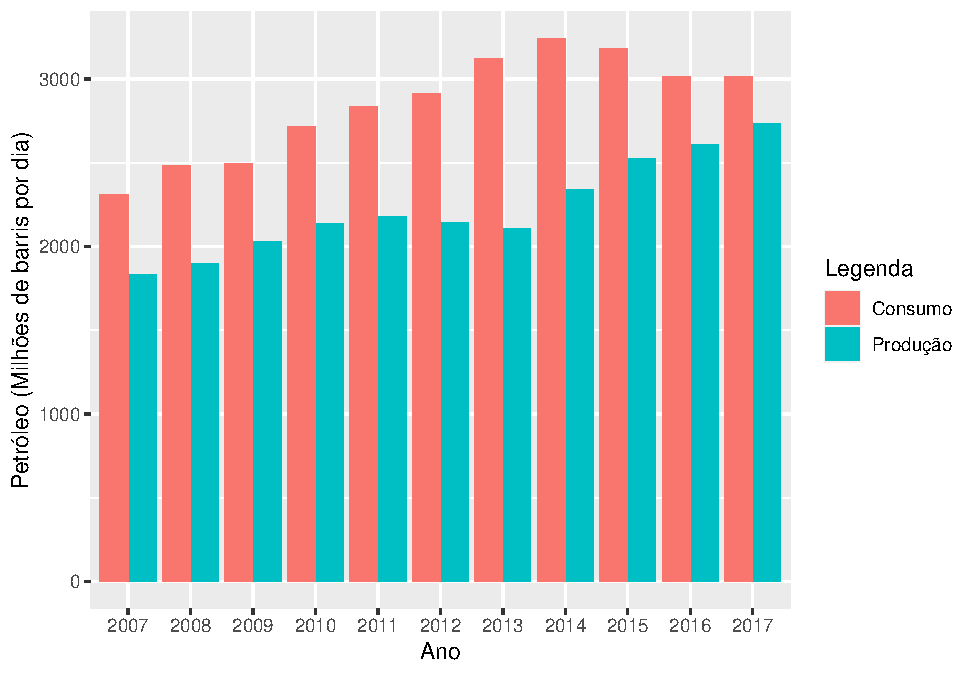
\includegraphics{01-cap01_files/figure-latex/prodcons-1.pdf}
\caption{\label{fig:prodcons}Produção e consumo de petróleo do Brasil nos períodos de 2007 a 2017.}
\end{figure}

O gráfico nos revela que o Brasil produz petróleo abaixo do que necessitaria para o consumo, de tal modo que a produção é 27,71\% a menos do que o consumo. Isso explica o porquê do Brasil como grande produtor de petróleo, ainda assim, necessita importar essa fonte de energia. Contudo, o gráfico não apresenta um resumo perfeito. Por exemplo, mesmo a produção de petróleo sendo mais baixa do que o consumo, o coeficiente de variação (assunto abordado no Capítulo \ref{chap:md} dessas dos dados dessas variáveis, são 12,99\% e 10,93\%, respectivamente, calculados de acordo com a Tabela \ref{tab:prodcons2}. Isso implica, que as variações da produção de petróleo são maiores do que as do consumo, no Brasil. Observe que essas últimas informações não podem ser vistas facilmente na Figura \ref{fig:prodcons}, mas juntamente com o auxílio das medidas numéricas (medidas de posição e dispersão) e as medidas gráficas, podemos complementar as informações, e assim, obter uma melhor descrição sobre essas informações.

\begin{table}

\caption{\label{tab:prodcons2}Volume, em MMbbl/d, da Produção e consumo de petróleo do Brasil nos períodos de 2007 a 2017.}
\centering
\begin{tabular}[t]{l|l|r}
\hline
Ano & Tipo & Volume\\
\hline
2007 & Produção & 1831\\
\hline
2008 & Produção & 1897\\
\hline
2009 & Produção & 2029\\
\hline
2010 & Produção & 2137\\
\hline
2011 & Produção & 2179\\
\hline
2012 & Produção & 2145\\
\hline
2013 & Produção & 2110\\
\hline
2014 & Produção & 2341\\
\hline
2015 & Produção & 2525\\
\hline
2016 & Produção & 2608\\
\hline
2017 & Produção & 2734\\
\hline
2007 & Consumo & 2308\\
\hline
2008 & Consumo & 2481\\
\hline
2009 & Consumo & 2498\\
\hline
2010 & Consumo & 2716\\
\hline
2011 & Consumo & 2839\\
\hline
2012 & Consumo & 2915\\
\hline
2013 & Consumo & 3124\\
\hline
2014 & Consumo & 3242\\
\hline
2015 & Consumo & 3181\\
\hline
2016 & Consumo & 3013\\
\hline
2017 & Consumo & 3017\\
\hline
\end{tabular}
\end{table}

Quando precisamos extender as informações contidas em um subconjunto (amostra) de dados para todo o conjunto (população), necessitamos de técnicas específicas dentro da estatística para garantir que estas informações sejam o mais verossímil possível. Técnicas estas são chamadas de Estatística Inferencial, definida a seguir.

\leavevmode\hypertarget{def:estinf}{}%
O estudo de técnicas que visam extender (extrapolar) a informação contida na amostra à população, chamamos de Estatística Inferencial ou Estatística Indutiva.

As técnicas abordadas na Estatística Inferencial estão relacionadas a determinar características (parâmetros) populacionais desconhecidas, ou até mesmo fazer afirmações sobre esses parâmetros.

A determinação de parâmetros por meio de características amostrais (estimadores) que chamamos de Estimação será abordado no Capítulo \ref{chap:teoest}. As afirmações realizadas sobre estes parâmetros, chamadas de hipóteses, serão estudadas no Capítulo \ref{chap:teodec}.

A Definição \protect\hyperlink{def:estinf}{1.3} nos mostra que por meio da Estatística, podemos tomar decisões sobre uma população através da amostra. Isso se faz necessário muitas vezes em uma pesquisa, devido a duas coisas preciosas: tempo e dinheiro. Muito embora, se tivermos acesso a todos os elementos de uma população, não se faz necessário o uso de técnicas da inferência estatística, e daí realizamos o que chamamos de Censo.

A forma de como se obter uma amostra é um dos passos mais importante em todo o processo da análise, uma vez que não adianta está com todo o aparato técnico se as informações contidas nessas amostra não são representativas da população. Para isso, temos uma área na estatística chamada Amostragem, que será responsável pelo desenvolvimento de métodos de como selecionar os elementos populacionais para compor a amostra de modo que as principais características contidas na população sejam preservadas na amostra. Esse assunto será estudado no Capítulo \ref{chap:sampling}.

Contudo, sabemos que entender uma população por um subconjunto desta, gera-se uma incerteza ou erro. A estatística tenta minimizar esse erro o máximo possível, isto é, reduzir as incertezas das informações contidas na amostra e extrapolar essas informações para a população. Para isso, usamos a probabilidade como suporte, assunto estudado nos Capítulos \ref{chap:cap5}, \ref{chap:cap6} e \ref{chap:cap8}.

\leavevmode\hypertarget{def:prob}{}%
A teoria matemática que estuda a incerteza de fenômenos aleatórios é chamada de probabilidade.

Os fenômenos aleatórios estão relacionados a situações que dificilmente saberemos com certeza do que pode acontecer. Por exemplo, se arremessarmos um dado de seis faces de tamanhos iguais e desejarmos saber a face superior desse dado antes do arremesso, não temos como afirmar com certeza qual o valor, se considerarmos as faces numerados de 1 a 6. Observe que, mesmo sabendo quais os valores das faces, não podemos afirmar com exatidão qual o valor da face superior antes do arremesso. Mas, por meio da probabilidade, podemos minimizar essa incerteza e dizer que há aproximadamete 17\% de chance de um número escolhido ocorrer.

Em nosso cotidiano, a probabilidade auxilia na decisão de um fabricante de cola de empreender uma grande publicidade no seu produto visando aumentar sua participação no mercado, ou na decisão de parar de imunizar pessoas com menos de vinte anos contra determinada doença, ou ainda na decisão de arriscar-se a atravessar uma rua no meio do quarteirão. Esses pequenos exemplos mostram a relação que a probabilidade tem com a inferência estatística, pois ela nos auxiliará a tomar decisões em procedimento inferencias tentando traduzir para a nossa linguagem do dia-a-dia.

Ao final dessas definições gerais, podemos mostrar uma ilustração, Figura \ref{fig:dispgerais}, que facilitará a compreensão do que abordamos nessa seção. Por fim, um último assunto estudado nesse livro, Capítulo \ref{chap:cor-reg}, será o estudo da correlação e regressão linear, quando estamos interessado em estudar a forma e o grau relação entre duas ou mais variáveis.

Todos esses assuntos estudaremos nos capítulos seguintes com um certo detalhamento, dando ênfase a exemplos práticos estudados em nosso campo de trabalho. Alguns Capítulos poderão conter uma seção chamada \emph{Aprofundamento}, com o intuito de apresentar uma maior profundidade sobre o tema estudado.

\begin{figure}

{\centering 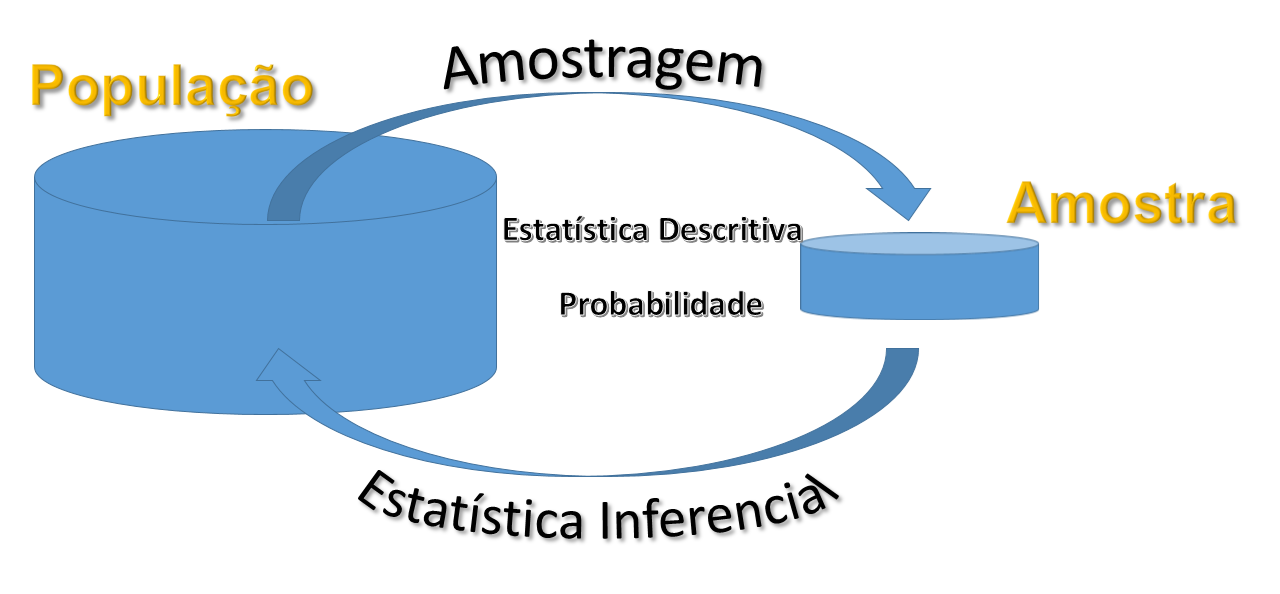
\includegraphics[width=1\linewidth]{images/book-epaec001-Disposicoes_Gerais} 

}

\caption{[Ilustração/Vídeo animado sobre as disposições gerais da Estatística.](https://youtu.be/mASLUwyaC5Q)}\label{fig:dispgerais}
\end{figure}

\hypertarget{subsec:est-pesqcient}{%
\subsection{Estatística na pesquisa científica}\label{subsec:est-pesqcient}}

O trabalho estatístico é parte integrante do método científico. Segundo \citet{silva2005}, definimos,

\leavevmode\hypertarget{def:prob}{}%
Um conjunto de regras e procedimentos para a obtenção de resultados, isto é, uma conclusão, sobre um determinado problema de uma pesquisa científica, é denominado de Método científico.

A pesquisa científica por sua vez, desenvolve conhecimentos para um saber mínimo de um determinado fenômeno estudado. A pesquisa científica se inicia a partir de um problema dentro da população em estudo. Por meio desse problema surgem diversas indagações.

\hypertarget{definiuxe7uxf5es-buxe1sicas}{%
\section{Definições básicas}\label{definiuxe7uxf5es-buxe1sicas}}

\hypertarget{tuxe9cnicas-de-somatuxf3rio}{%
\section{Técnicas de somatório}\label{tuxe9cnicas-de-somatuxf3rio}}

\hypertarget{normas-de-arredondamento}{%
\subsection{Normas de arredondamento}\label{normas-de-arredondamento}}

\hypertarget{exercuxedcios-prospostos}{%
\section*{Exercícios prospostos}\label{exercuxedcios-prospostos}}


\hypertarget{chap:coad}{%
\chapter{Coleta, organização e apresentação dos dados}\label{chap:coad}}

\hypertarget{chap:mp}{%
\chapter{Medidas de posição}\label{chap:mp}}

\hypertarget{introduuxe7uxe3o-1}{%
\section{Introdução}\label{introduuxe7uxe3o-1}}

\hypertarget{muxe9dia}{%
\section{Média}\label{muxe9dia}}

\hypertarget{mediana}{%
\section{Mediana}\label{mediana}}

\hypertarget{moda}{%
\section{Moda}\label{moda}}

\hypertarget{chap:md}{%
\chapter{Medidas de dispersão}\label{chap:md}}

\hypertarget{introduuxe7uxe3o-2}{%
\section{Introdução}\label{introduuxe7uxe3o-2}}

\hypertarget{amplitude-total}{%
\section{Amplitude total}\label{amplitude-total}}

\hypertarget{variuxe2ncia}{%
\section{Variância}\label{variuxe2ncia}}

\hypertarget{desvio-padruxe3o}{%
\section{Desvio padrão}\label{desvio-padruxe3o}}

\hypertarget{coeficiente-de-variauxe7uxe3o}{%
\section{Coeficiente de Variação}\label{coeficiente-de-variauxe7uxe3o}}

\hypertarget{erro-padruxe3o-da-muxe9dia}{%
\section{Erro padrão da média}\label{erro-padruxe3o-da-muxe9dia}}

\hypertarget{chap:cap5}{%
\chapter{Probabilidades}\label{chap:cap5}}

\hypertarget{conceitos-buxe1sicos}{%
\section{Conceitos básicos}\label{conceitos-buxe1sicos}}

\hypertarget{leis-buxe1sicas-da-teoria-de-conjuntos}{%
\subsection{Leis básicas da teoria de conjuntos}\label{leis-buxe1sicas-da-teoria-de-conjuntos}}

\hypertarget{teoremas-cluxe1ssicos-da-teoria-de-conjuntos}{%
\subsection{Teoremas clássicos da teoria de conjuntos}\label{teoremas-cluxe1ssicos-da-teoria-de-conjuntos}}

\hypertarget{definiuxe7uxf5es-de-probabilidades}{%
\section{Definições de probabilidades}\label{definiuxe7uxf5es-de-probabilidades}}

\hypertarget{propriedades}{%
\section{Propriedades}\label{propriedades}}

\hypertarget{regra-de-adiuxe7uxe3o-de-probabilidades}{%
\subsection{Regra de adição de probabilidades}\label{regra-de-adiuxe7uxe3o-de-probabilidades}}

\hypertarget{probabilidade-de-um-evento-complementar}{%
\subsection{Probabilidade de um evento complementar}\label{probabilidade-de-um-evento-complementar}}

\hypertarget{eventos-independentes-e-probabilidade-condicional}{%
\section{Eventos independentes e probabilidade condicional}\label{eventos-independentes-e-probabilidade-condicional}}

\hypertarget{teorema-de-bayes}{%
\section{Teorema de Bayes}\label{teorema-de-bayes}}

\hypertarget{variuxe1vel-aleatuxf3ria}{%
\section{Variável Aleatória}\label{variuxe1vel-aleatuxf3ria}}

\hypertarget{distribuiuxe7uxe3o-de-probabilidade-discreta}{%
\section{Distribuição de probabilidade discreta}\label{distribuiuxe7uxe3o-de-probabilidade-discreta}}

\hypertarget{distribuiuxe7uxe3o-de-probabilidade-contuxednua}{%
\section{Distribuição de probabilidade contínua}\label{distribuiuxe7uxe3o-de-probabilidade-contuxednua}}

\hypertarget{funuxe7uxe3o-de-distribuiuxe7uxe3o-acumulada-fda}{%
\section{Função de distribuição acumulada (FDA)}\label{funuxe7uxe3o-de-distribuiuxe7uxe3o-acumulada-fda}}

\hypertarget{fda-para-x-discreta}{%
\subsection{\texorpdfstring{FDA para \(X\) discreta}{FDA para X discreta}}\label{fda-para-x-discreta}}

\hypertarget{fda-para-x-contuxednua}{%
\subsection{\texorpdfstring{FDA para \(X\) contínua}{FDA para X contínua}}\label{fda-para-x-contuxednua}}

\hypertarget{esperanuxe7a-matemuxe1tica-e-variuxe2ncia}{%
\section{Esperança matemática e variância}\label{esperanuxe7a-matemuxe1tica-e-variuxe2ncia}}

\hypertarget{esperanuxe7a-matemuxe1tica}{%
\subsection{Esperança matemática}\label{esperanuxe7a-matemuxe1tica}}

\hypertarget{mediana-1}{%
\subsection{Mediana}\label{mediana-1}}

\hypertarget{moda-1}{%
\subsection{Moda}\label{moda-1}}

\hypertarget{variuxe2ncia-e-desvio-padruxe3o}{%
\subsection{Variância e desvio padrão}\label{variuxe2ncia-e-desvio-padruxe3o}}

\hypertarget{exercuxedcios-propostos}{%
\section*{Exercícios propostos}\label{exercuxedcios-propostos}}


\hypertarget{chap:cap6}{%
\chapter{Distribuições de probabilidade}\label{chap:cap6}}

\hypertarget{introduuxe7uxe3o-3}{%
\section{Introdução}\label{introduuxe7uxe3o-3}}

\hypertarget{distribuiuxe7uxf5es-discretas-de-probabilidades}{%
\section{Distribuições discretas de probabilidades}\label{distribuiuxe7uxf5es-discretas-de-probabilidades}}

\hypertarget{distribuiuxe7uxe3o-bernoulli}{%
\subsection{Distribuição Bernoulli}\label{distribuiuxe7uxe3o-bernoulli}}

\hypertarget{distribuiuxe7uxe3o-binomial}{%
\subsection{Distribuição Binomial}\label{distribuiuxe7uxe3o-binomial}}

\hypertarget{distribuiuxe7uxe3o-poisson}{%
\subsection{Distribuição Poisson}\label{distribuiuxe7uxe3o-poisson}}

\hypertarget{relauxe7uxe3o-entre-a-distribuiuxe7uxe3o-binomial-e-poisson}{%
\subsection{Relação entre a distribuição Binomial e Poisson}\label{relauxe7uxe3o-entre-a-distribuiuxe7uxe3o-binomial-e-poisson}}

\hypertarget{distribuiuxe7uxf5es-contuxednuas-de-probabilidades}{%
\section{Distribuições contínuas de probabilidades}\label{distribuiuxe7uxf5es-contuxednuas-de-probabilidades}}

\hypertarget{distribuiuxe7uxe3o-normal}{%
\subsection{Distribuição normal}\label{distribuiuxe7uxe3o-normal}}

\hypertarget{distribuiuxe7uxe3o-normal-padruxe3o}{%
\subsubsection{Distribuição normal padrão}\label{distribuiuxe7uxe3o-normal-padruxe3o}}

\hypertarget{chap:sampling}{%
\chapter{Amostragem}\label{chap:sampling}}

\hypertarget{introduuxe7uxe3o-4}{%
\section{Introdução}\label{introduuxe7uxe3o-4}}

\hypertarget{amostragem-nuxe3o-probabiluxedstica-e-probabiluxedstica}{%
\section{Amostragem não-probabilística e probabilística}\label{amostragem-nuxe3o-probabiluxedstica-e-probabiluxedstica}}

\hypertarget{tuxe9cnicas-de-amostragem-probabiluxedstica}{%
\section{Técnicas de amostragem probabilística}\label{tuxe9cnicas-de-amostragem-probabiluxedstica}}

\hypertarget{chap:cap8}{%
\chapter{Distribuição de amostragem}\label{chap:cap8}}

\hypertarget{introduuxe7uxe3o-5}{%
\section{Introdução}\label{introduuxe7uxe3o-5}}

\hypertarget{distribuiuxe7uxe3o-de-amostragem-da-muxe9dia}{%
\section{Distribuição de amostragem da média}\label{distribuiuxe7uxe3o-de-amostragem-da-muxe9dia}}

\hypertarget{distribuiuxe7uxe3o-de-amostragem-de-proporuxe7uxf5es}{%
\section{Distribuição de amostragem de proporções}\label{distribuiuxe7uxe3o-de-amostragem-de-proporuxe7uxf5es}}

\hypertarget{distribuiuxe7uxe3o-de-amostragem-de-diferenuxe7a-entre-muxe9dias}{%
\section{Distribuição de amostragem de diferença entre médias}\label{distribuiuxe7uxe3o-de-amostragem-de-diferenuxe7a-entre-muxe9dias}}

\hypertarget{distribuiuxe7uxf5es-amostrais-para-variuxe2ncia}{%
\section{Distribuições amostrais para variância}\label{distribuiuxe7uxf5es-amostrais-para-variuxe2ncia}}

\hypertarget{chap:teoest}{%
\chapter{Teoria de estimação}\label{chap:teoest}}

\hypertarget{introduuxe7uxe3o-6}{%
\section{Introdução}\label{introduuxe7uxe3o-6}}

\hypertarget{conceitos-buxe1sicos-1}{%
\section{Conceitos básicos}\label{conceitos-buxe1sicos-1}}

\hypertarget{tipos-de-estimador}{%
\section{Tipos de estimador}\label{tipos-de-estimador}}

\hypertarget{propriedades-de-um-estimador}{%
\section{Propriedades de um estimador}\label{propriedades-de-um-estimador}}

\hypertarget{estimauxe7uxe3o-por-ponto}{%
\section{Estimação por ponto}\label{estimauxe7uxe3o-por-ponto}}

\hypertarget{estimauxe7uxe3o-por-intervalo}{%
\section{Estimação por intervalo}\label{estimauxe7uxe3o-por-intervalo}}

\hypertarget{intervalo-de-confianuxe7a-para-a-muxe9dia}{%
\subsection{Intervalo de confiança para a média}\label{intervalo-de-confianuxe7a-para-a-muxe9dia}}

\hypertarget{intervalo-de-confianuxe7a-para-a-variuxe2ncia}{%
\subsection{Intervalo de confiança para a variância}\label{intervalo-de-confianuxe7a-para-a-variuxe2ncia}}

\hypertarget{intervalo-de-confianuxe7a-de-confianuxe7a-para-a-diferenuxe7a-entre-muxe9dias}{%
\subsection{Intervalo de confiança de confiança para a diferença entre médias}\label{intervalo-de-confianuxe7a-de-confianuxe7a-para-a-diferenuxe7a-entre-muxe9dias}}

\hypertarget{dimensionamento-de-amostras}{%
\section{Dimensionamento de amostras}\label{dimensionamento-de-amostras}}

\hypertarget{chap:teodec}{%
\chapter{Teoria da decisão}\label{chap:teodec}}

\hypertarget{introduuxe7uxe3o-7}{%
\section{Introdução}\label{introduuxe7uxe3o-7}}

\hypertarget{teste-de-hipuxf3teses}{%
\section{Teste de hipóteses}\label{teste-de-hipuxf3teses}}

\hypertarget{erros-tipo-i-e-ii}{%
\section{Erros tipo I e II}\label{erros-tipo-i-e-ii}}

\hypertarget{teste-unilateral-e-bilateral}{%
\section{Teste unilateral e bilateral}\label{teste-unilateral-e-bilateral}}

\hypertarget{passos-para-a-construuxe7uxe3o-de-um-teste-de-hipuxf3tese}{%
\section{Passos para a construção de um teste de hipótese}\label{passos-para-a-construuxe7uxe3o-de-um-teste-de-hipuxf3tese}}

\hypertarget{testes-de-hipuxf3teses-para-a-muxe9dia}{%
\section{Testes de hipóteses para a média}\label{testes-de-hipuxf3teses-para-a-muxe9dia}}

\hypertarget{testes-de-hipuxf3teses-para-a-proporuxe7uxe3o}{%
\section{Testes de hipóteses para a proporção}\label{testes-de-hipuxf3teses-para-a-proporuxe7uxe3o}}

\hypertarget{testes-de-hipuxf3teses-para-a-variuxe2ncia}{%
\section{Testes de hipóteses para a variância}\label{testes-de-hipuxf3teses-para-a-variuxe2ncia}}

\hypertarget{testes-de-hipuxf3teses-para-a-diferenuxe7a-entre-duas-muxe9dias}{%
\section{Testes de hipóteses para a diferença entre duas médias}\label{testes-de-hipuxf3teses-para-a-diferenuxe7a-entre-duas-muxe9dias}}

\hypertarget{chap:cor-reg}{%
\chapter{Correlação e regressão linear simples}\label{chap:cor-reg}}

\hypertarget{introduuxe7uxe3o-8}{%
\section{Introdução}\label{introduuxe7uxe3o-8}}

\hypertarget{correlauxe7uxe3o-linear}{%
\section{Correlação linear}\label{correlauxe7uxe3o-linear}}

\hypertarget{coeficiente-de-correlauxe7uxe3o-linear}{%
\subsection{Coeficiente de correlação linear}\label{coeficiente-de-correlauxe7uxe3o-linear}}

\hypertarget{teste-de-hipuxf3teses-acerca-do-coeficiente-de-correlauxe7uxe3o-linear}{%
\subsection{Teste de hipóteses acerca do coeficiente de correlação linear}\label{teste-de-hipuxf3teses-acerca-do-coeficiente-de-correlauxe7uxe3o-linear}}

\hypertarget{regressuxe3o-linear-simples}{%
\section{Regressão linear simples}\label{regressuxe3o-linear-simples}}

\hypertarget{modelo}{%
\subsection{Modelo}\label{modelo}}

\hypertarget{estimauxe7uxe3o-dos-paruxe2metros-do-modelo}{%
\subsection{Estimação dos parâmetros do modelo}\label{estimauxe7uxe3o-dos-paruxe2metros-do-modelo}}

\hypertarget{teste-de-hipuxf3teses-para-o-modelo-de-regressuxe3o}{%
\subsection{Teste de hipóteses para o modelo de regressão}\label{teste-de-hipuxf3teses-para-o-modelo-de-regressuxe3o}}

\hypertarget{medidas-de-adequauxe7uxe3o-do-modelo}{%
\subsection{Medidas de adequação do modelo}\label{medidas-de-adequauxe7uxe3o-do-modelo}}

\hypertarget{apuxeandice-a---introduuxe7uxe3o-ao-r}{%
\chapter*{Apêndice A - Introdução ao R}\label{apuxeandice-a---introduuxe7uxe3o-ao-r}}


  \bibliography{epaec.bib}

\end{document}
